\section{Kết quả của các kỹ thuật cải tiến}
\subsection{Mô hình cải tiến}
Có thể thấy được cả hai mô hình đều có thể hội tụ sao 10 epoch, nhưng mô hình cải tiến hội tụ nhanh hơn và có loss thấp hơn so với mô hình cũ. Điều này có thể thấy rõ ở hình \ref{fig:loss_model}. Mô hình cải tiến có loss thấp hơn mô hình cũ sau 10 epoch. Điều này có thể hiểu là mô hình cải tiến học nhanh hơn và hiệu quả hơn so với mô hình cũ.

\begin{figure}[H]
    \centering
    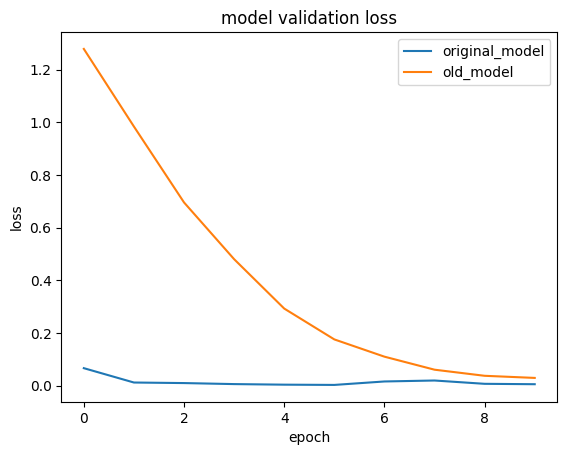
\includegraphics[width=0.8\textwidth]{Images/Improvement results/old_new_loss.png}
    \caption{Loss của cả hai mô hình }
    \label{fig:loss_model}
\end{figure}

Điều này có thể thấy rõ hơn ở confusion matrix của cả hai mô hình ở trên tập test. Mô hình cải tiến có thể dự đoán chính xác đa số các mẫu trong tập test trong khi mô hình cũ dự đoán sai một số mẫu trong tập test.

\begin{figure}[H]
    \centering
    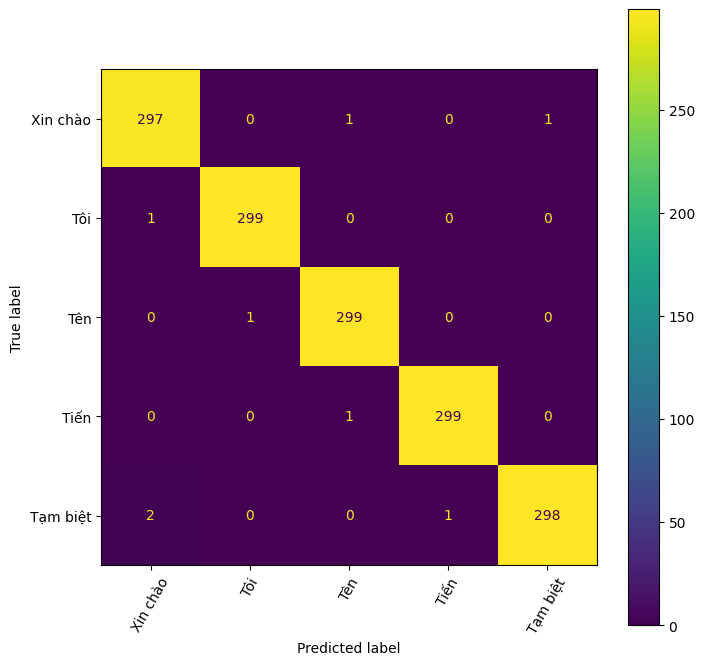
\includegraphics[width=0.8\textwidth]{Images/Improvement results/new_confusion_matrix.png}
    \caption{Confusion matrix của mô hình mới}
    \label{fig:confusion_matrix_new}
\end{figure}

\begin{figure}[H]
    \centering
    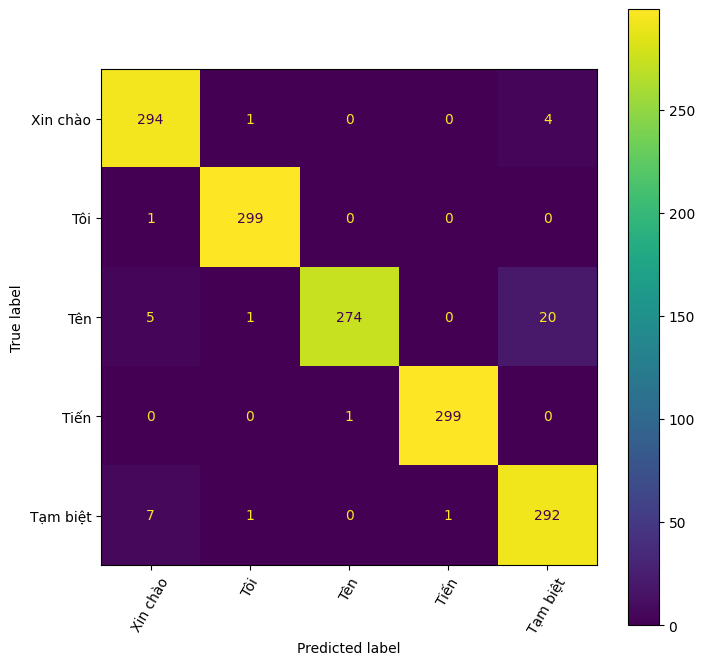
\includegraphics[width=0.8\textwidth]{Images/Improvement results/old_confusion_matrix.png}
    \caption{Confusion matrix của mô hình cũ}
    \label{fig:confusion_matrix_old}
\end{figure}

Không những vậy mô hình cũng có confidence trung bình cho những mẫu đoán đúng cao hơn so với mô hình cũ. Điều này có thể thấy rõ ở hình \ref{fig:confidence_model}. Mô hình cải tiến có confidence trung bình cho những mẫu đoán đúng cao hơn mô hình cũ. 

\begin{figure}[H]
    \centering
    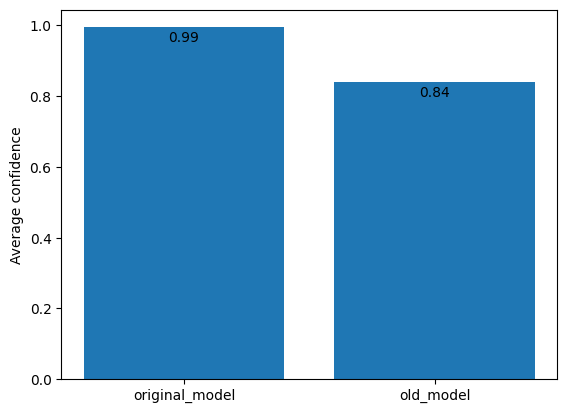
\includegraphics[width=0.8\textwidth]{Images/Improvement results/old_new_confidence.png}
    \caption{Confidence của cả hai mô hình}
    \label{fig:confidence_model}
\end{figure}

Kiểm nghiệm thực tế cũng cho thấy mô hình cải tiến hoạt động tốt hơn so với mô hình cũ. Mô hình cải tiến có thể dự đoán chính xác hơn 90\%  trong khi mô hình cũ chỉ có thể dự đoán chính xác khoảng 70\% và cũng như có confidence cao hơn trong các lần dự đoán.

\subsection{Làm giàu dữ liệu}
\subsubsection{Data augmentation}
Nhóm chọn 4 kỹ thuật làm giàu dữ liệu là: Jitter, Shift, Scale và Magnitude Warp.

\begin{figure}[H]
    \centering
    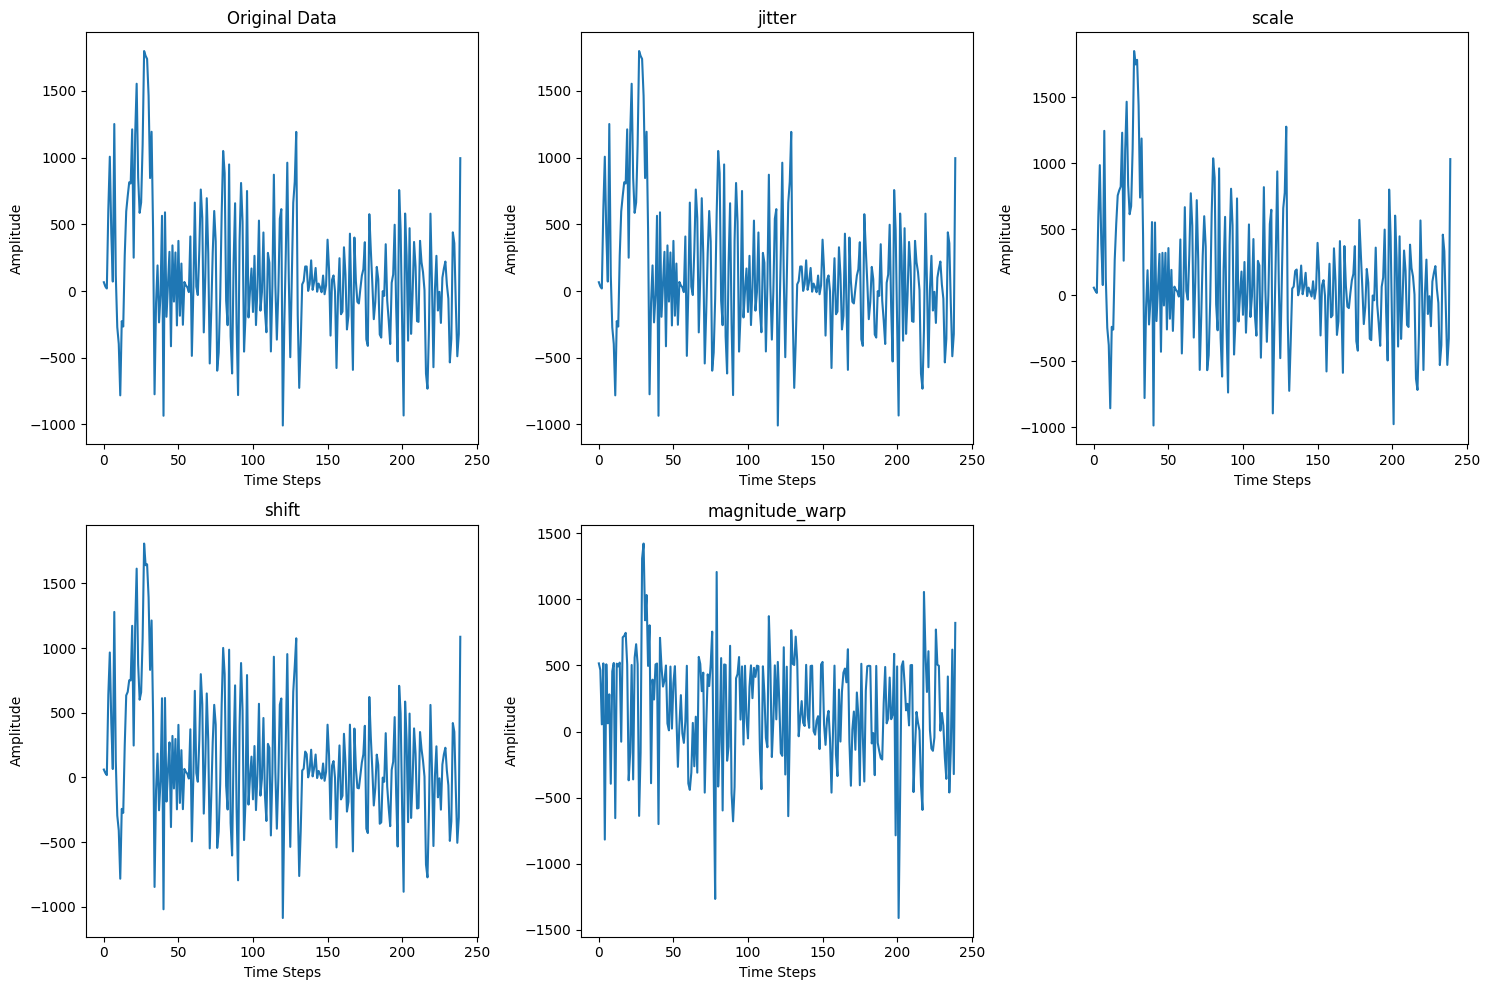
\includegraphics[width=1\textwidth]{Images/Improvement results/data_augmentation.png}
    \caption{Data augmentation}
    \label{fig:data_augmentation}
\end{figure}

Với mỗi kỹ thuật làm giàu dữ liệu, nhóm đã ghép 2 kỹ thuật lại với nhau để tạo ra 6 cặp kỹ thuật làm giàu dữ liệu. 
Sau cùng dữ liệu có kích thước gấp 10 lần dữ liệu ban đầu.

\begin{figure}[H]
    \centering
    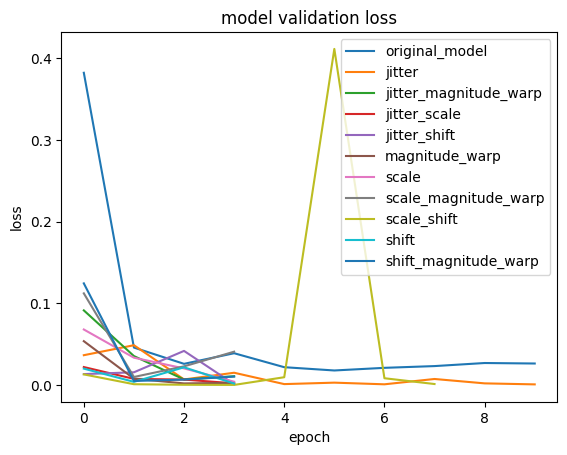
\includegraphics[width=0.8\textwidth]{Images/Improvement results/data_augmentation_loss.png}
    \caption{Loss của các kỹ thuật làm giàu dữ liệu}
    \label{fig:data_augmentation_loss}
\end{figure}



Nhìn chung kết quả của các kỹ thuật đều giúp mô hình hội tụ nhanh hơn khi sử dụng tập dữ liệu ban đầu. Bởi vì mô hình mới với dữ liệu ban đầu đã làm rất tốt nên việc làm giàu dữ liệu không thể hiện rõ ở mặt độ chính xác của mô hình. Tuy nhiên, có một số kỹ thuật làm giàu dữ liệu giúp mô hình hội tụ nhanh hơn so với dữ liệu ban đầu và có loss thấp hơn ví dụ như jitter.

\begin{figure}[H]
    \centering
    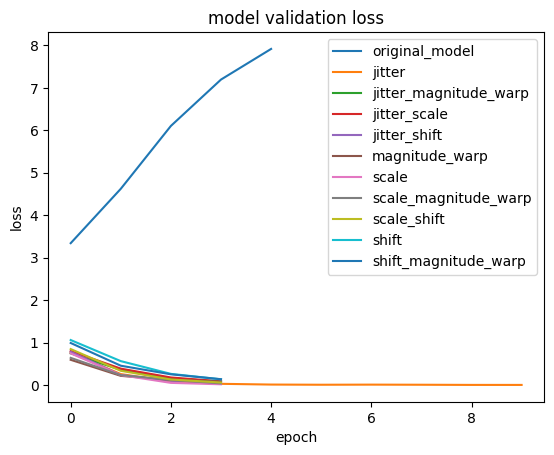
\includegraphics[width=0.8\textwidth]{Images/Improvement results/old_data_augmentation_loss.png}
    \caption{Loss của mô hình cũ với dữ liệu đã làm giàu}
    \label{fig:old_data_augmentation_loss}
\end{figure}

Điều này được thể hiện rõ hơn khi nhóm áp dụng tập dữ liệu đã làm giàu vào mô hình cũ. Mô hình cũ với dữ liệu đã làm giàu có thể hội tụ nhanh và có loss thấp hơn so với mô hình cũ với dữ liệu ban đầu với jitter là mô hình có loss thấp nhất - điều tương tự đã quan sát được ở mô hình mới.

\begin{figure}[H]
    \centering
    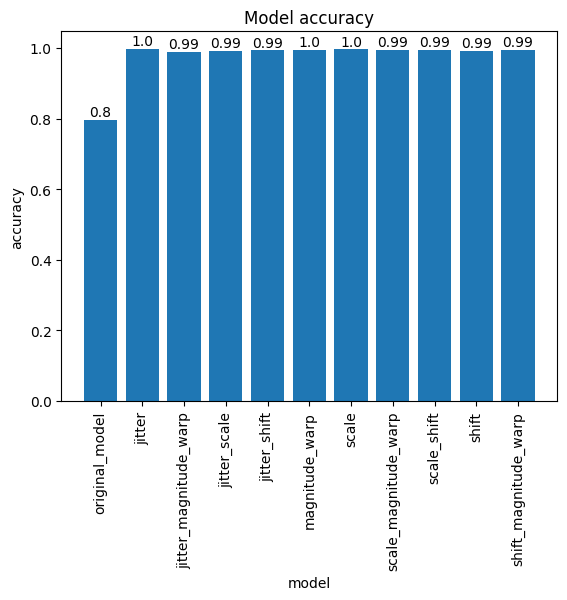
\includegraphics[width=0.8\textwidth]{Images/Improvement results/old_data_augmentation_accuracy.png}
    \caption{Accuracy của mô hình cũ với dữ liệu đã làm giàu}
    \label{fig:old_data_augmentation_accuracy}
\end{figure}

Với mô hình cũ, dữ liệu đã làm giàu giúp mô hình có độ chính xác cao hơn so với dữ liệu ban đầu với độ cải thiện từ 80\% lên 100\% đối với tập test. Nhìn chung các mô hình với dữ liệu đã làm giàu đều có độ chính xác cải thiện rõ rệt so với dữ liệu ban đầu. Kiểm nghiệm thực tế cũng cho thấy cải thiện từ 5\% đến 10\% so với dữ liệu ban đầu.

\subsection{Transfer learning}
Bước đầu thực hiện huấn luyện mô hình với tập dữ liệu ASL Data Glove giữ nguyên 11 đặc trưng cho kết quả dự đoán của mô hình trên tập validation là gần mức 0.8. 

\begin{figure}[H]
    \centering
    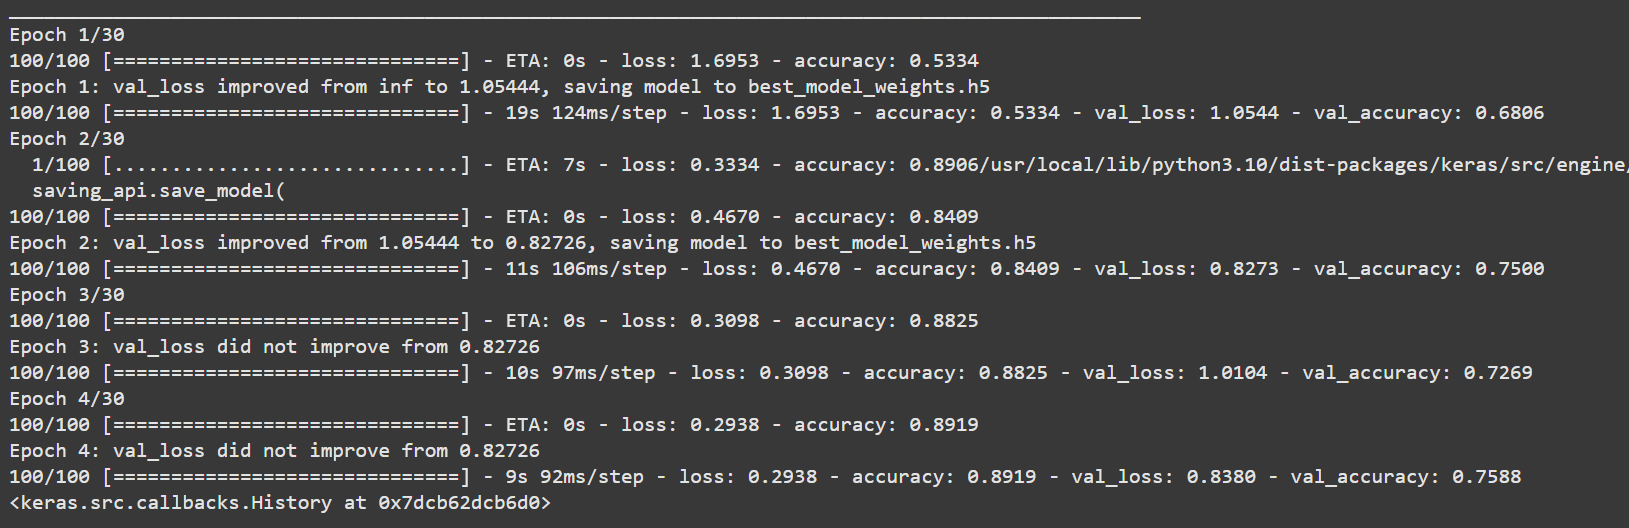
\includegraphics[width=1.1\textwidth]{Images/Improvement results/transfer_learning_training_result_full_class.png}
    \caption{Transfer learning với 11 đặc trưng}
    \label{fig:transfer_learning_training_result_full_class}
\end{figure}


Sau đó, nhóm thực hiện biến đổi dữ liệu để phù hợp với tính chất dữ liệu của nhóm và cắt giảm từ 11 xuống còn 7 đặc trưng. Kết quả huấn luyện của mô hình giảm rõ rệt so với mô hình với 11 đặc trưng. Điều này có thể dự đoán được vì với 40 nhãn của tập dữ liệu ASL Data Glove, mô hình cần nhiều đặc trưng hơn để có thể dự đoán chính xác hơn.

\begin{figure}[H]
    \centering
    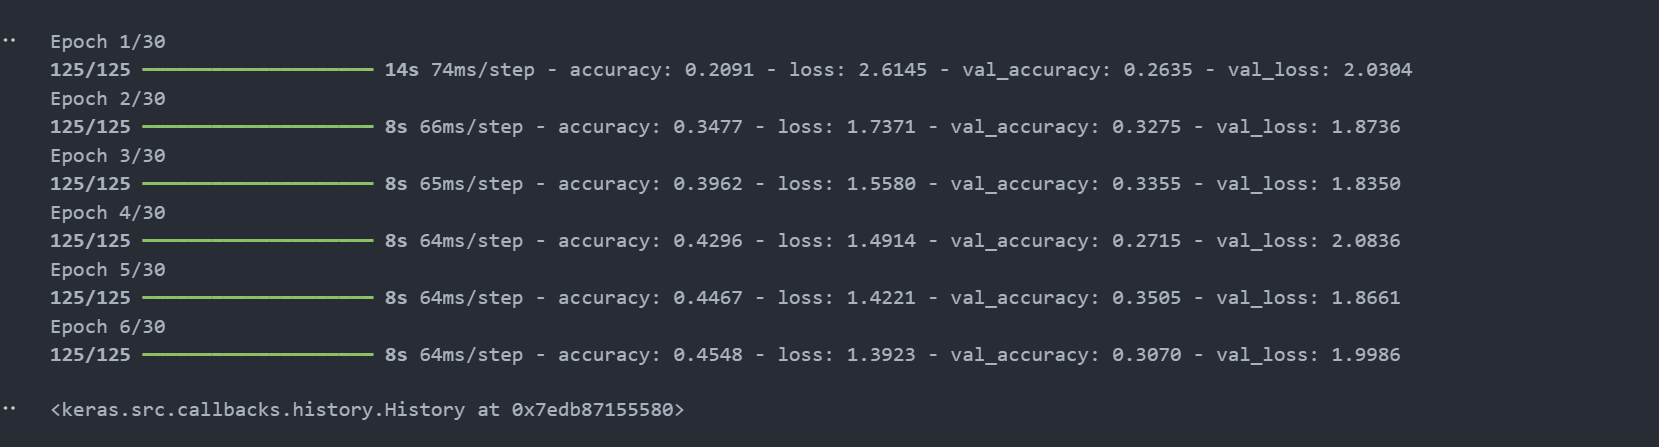
\includegraphics[width=1.1\textwidth]{Images/Improvement results/transfer_learning_training_result.png}
    \caption{Transfer learning với 7 đặc trưng}
    \label{fig:transfer_learning_training_result_7_class}
\end{figure}

Sau khi chuyển weight của mô hình đã được huấn luyện với tập dữ liệu ASL Data Glove sang mô hình mới, quá trình huấn luyện mô hình transfer learning có thấy mô hình transfer learning hội tụ nhanh hơn so với mô hình mới, loss cũng thấp hơn so với mô hình ban đầu. 

\begin{figure}[H]
    \centering
    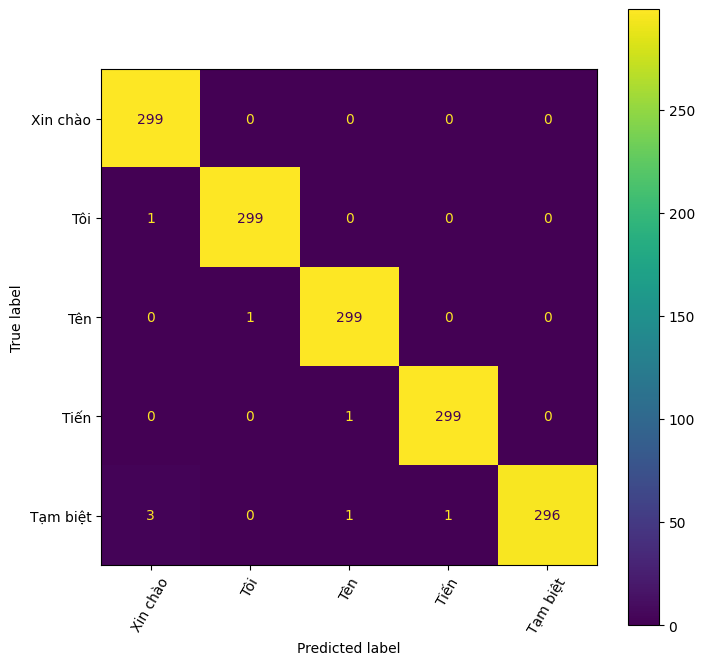
\includegraphics[width=0.8\textwidth]{Images/Improvement results/transfer_learning_confusion_matrix.png}
    \caption{So sánh transfer learning và mô hình mới}
    \label{fig:transfer_learning_training_result_compare}
\end{figure}

Kết quả của mô hình transfer learning ở tập test cũng cho thấy mô hình có thể dự đoán đúng nhiều hơn so với mô hình mới ban đầu. Tuy nhiên sự khác biệt là không lớn (<10 mẫu) và kiểm nghiệm thực tế cũng cho thấy sai khác <5\% giữa mô hình mới và mô hình transfer learning.

% Data được thu thập sau đó được phân bổ với tỉ lệ 80-20, 80\% lượng data được sử dụng để train mô hình, 20\% được sử dụng để kiểm tra kết quả sau khi huấn luyện

% Chúng ta không thể đánh giá kỹ năng của mô hình chỉ từ một lần đánh giá.
% Nguyên nhân là mạng nơ-ron là ngẫu nhiên, có nghĩa là một cấu hình mô hình cụ thể khác nhau sẽ xuất hiện khi đào tạo cùng một cấu hình mô hình trên cùng một dữ liệu. Điều này là một đặc trưng của mạng, vì nó mang lại khả năng thích ứng cho mô hình, nhưng yêu cầu một quá trình đánh giá mô hình phức tạp hơn.

% Chúng ta sẽ lặp lại việc đánh giá mô hình nhiều lần, sau đó tóm tắt hiệu suất của mô hình qua từng lần chạy đó. chúng ta có thể gọi hàm evaluate\_model() tổng cộng 5 lần.Điều này sẽ dẫn đến một tập hợp các điểm đánh giá mô hình cần được tóm tắt.'\\

% \begin{lstlisting}
% >#1: 90.058
% >#2: 85.918
% >#3: 90.974
% >#4: 89.515
% >#5: 90.159
% >#6: 91.110
% >#7: 89.718
% >#8: 90.295
% >#9: 89.447
% >#10: 90.024

% [90.05768578215134, 85.91788259246692, 90.97387173396675, 89.51476077366813, 90.15948422124194, 91.10960298608755, 89.71835765184933, 90.29521547336275, 89.44689514760775, 90.02375296912113]

% Accuracy: 89.722% (+/-1.371)

% \end{lstlisting}
% Cuối cùng, mẫu các điểm đánh giá được in ra, tiếp theo là giá trị trung bình và độ lệch chuẩn. Chúng ta có thể thấy rằng mô hình đã hoạt động tốt, đạt được độ chính xác phân loại khoảng 89,7\% khi được huấn luyện trên dữ liệu thô, với độ lệch chuẩn là khoảng 1,3. Đây là một kết quả tốt ! 
% \subsection{}

% Dựa vào số động tác thực hiện và số lần mô hình xác định chính xác, cho thấy mô hình chỉ đạt kết quả khoảng 70\%: \\

% Kết quả này được thực hiện như sau:\\
% \begin{itemize}
%     \item Một động tác được duy trì trong 2.4s bằng với số frame dữ liệu được gửi đến mô hình để dự đoán
%     \item Thực hiện động tác với label 7 và 9 vì hai động tác này có data frame khá tương đồng nhau,  trong 1 phút bằng với 25 lần mô hình gửi đến model kết quả cho thấy chỉ dự đoán được 18 lần với label 7 và 17 lần với label 9
% \end{itemize}
% Những động tác có data frame khác biệt nhau ví dự như label 5 và label 0 cho ra kết quả khá chính xác, lên đến hơn 90\% dựa vào cách tính trên


